\documentclass[12pt]{article}

\usepackage{sbc-template}
\usepackage{graphicx,url}
\usepackage[utf8]{inputenc}
\usepackage[brazil]{babel}
\usepackage{booktabs}
\usepackage[most]{tcolorbox}
\usepackage{subfigure}
\usepackage{subcaption}
\usepackage{float}
\definecolor{block-gray}{gray}{0.85}
%\usepackage[latin1]{inputenc}

\sloppy

\title{Desenvolvimento de Aplicativo Móvel para Contagem de Produtos com Coletores de Dados: Otimização da Correção de Saldo de Estoque}

\author{Ivaney Vieira de Sales\inst{1}, Ricardo Martins Ramos\inst{2}}

\address{Instituto Federal de Educação, Ciência e Tecnologia do Piauí\\
R. Álvaro Mendes, 94 -- Centro (Sul) -- 64.000-040 -- Teresina -- PI -- Brasil 
\nextinstitute
Instituto Federal de Educação, Ciência e Tecnologia do Piauí\\
R. Álvaro Mendes, 94 -- Centro (Sul) -- 64.000-040 -- Teresina -- PI -- Brasil
}

\begin{document} 

\maketitle

\begin{resumo}

  Este trabalho visa desenvolver um aplicativo de gestão de inventário para otimizar o controle e a organização de estoque em depósitos. No cenário dinâmico do varejo brasileiro, os erros de estoque são um desafio significativo, impactando a eficiência dos processos e a satisfação do cliente. A implementação de inventários cíclicos melhora a precisão e gestão dos estoques, promovendo a eficiência operacional e a redução de custos. O aplicativo proposto possui dois módulos: um para auditores, que permite a contagem de produtos via dispositivos móveis, e outro para gerentes, oferecendo ferramentas abrangentes para cadastro, gestão de lotes, auditoria e geração de relatórios. Com integração a sistemas existentes, rastreamento de movimentação de produtos e suporte a leitura de códigos de barras, o aplicativo visa maximizar a eficiência e transparência no gerenciamento de estoque. Treinamentos e suporte técnico contínuos garantem a adoção eficaz do sistema, destacando-se como uma solução essencial para empresas de diversos setores.

\textbf{Palavras-chave}: Gestão de Inventário. Eficiência Operacional. Auditoria de Estoque. Aplicativo Móvel.
  
\end{resumo}

\begin{abstract}

  This work aims to develop an inventory management application to optimize the control and organization of stock in warehouses. In Brazil’s dynamic retail landscape, inventory errors are a significant challenge, impacting process efficiency and customer satisfaction. Implementing cyclical inventories improves stock accuracy and management, promoting operational efficiency and reducing costs. The proposed application has two modules: one for auditors, which allows product counting via mobile devices, and another for managers, offering comprehensive tools for registration, batch management, auditing and report generation. With integration into existing systems, product movement tracking and support for barcode scanning, the application aims to maximize efficiency and transparency in stock management. Ongoing training and technical support ensure effective adoption of the system, making it an essential solution for companies in a wide range of sectors.

\textbf{Keywords}: Inventory Management. Operational efficiency. Stock Audit. Mobile Application.

\end{abstract}

\section{Introdução}

% apresentar o problema que o aplicativo visa solucionar

No cenário dinâmico do varejo brasileiro, os erros de estoque representam uma questão crucial que pode impactar negativamente a eficiência operacional e a satisfação do cliente. O desafio reside na necessidade de manter um equilíbrio delicado entre a oferta e a demanda, garantindo que os produtos certos estejam disponíveis no momento certo. Nesse contexto, a implementação de um processo de inventário assume um papel estratégico e indispensável.

% Um breve referencial teórico

Realizar inventários é crucial para garantir a precisão das informações de saldo de estoque. Erros no registro de transações e no manuseio físico do estoque podem causar discrepâncias entre o estoque registrado e o real, que só são corrigidas durante verificações físicas esporádicas. Na prática, diversas transações aumentam a possibilidade de erros, resultando em registros imprecisos de estoque. As causas comuns incluem erros de digitação, contagem incorreta de produtos, falhas em registrar corretamente produtos danificados ou destruídos, retirada e retorno de itens sem a devida correção nos registros, atrasos na atualização dos registros após transações e roubos de estoque, frequentes no varejo e também presentes em ambientes industriais e comerciais \cite{nigel}.

Segundo a pesquisa realizada por \cite{silva}, a adoção de inventários cíclicos representa uma prática estratégica que não apenas melhora a acurácia e a gestão dos estoques, mas também promove a eficiência operacional e a redução de custos, fortalecendo a competitividade da empresa no mercado.

% Objetivo final da introdução

Um aplicativo de gestão de inventário emerge como uma solução indispensável para o controle e a organização eficaz do estoque em depósitos. Projetado cuidadosamente para otimizar o gerenciamento de produtos, contagem física, auditoria e geração de relatórios, este aplicativo abrange diversas necessidades cruciais dos gerentes, auditores e equipes de controle de inventário. Estruturado em dois módulos distintos, o aplicativo para dispositivo móvel que proporciona funcionalidades específicas para auditores fazerem as contagem de produtos no depósito, enquanto outro atende às demandas do gerente de inventário.

O módulo destinado aos auditores é implementado em dispositivos móveis, como coletores de dados, facilitando a execução da contagem física dos produtos nos diversos lotes do depósito. Por meio de uma interface intuitiva, os auditores podem realizar suas atividades de forma eficiente, assegurando a precisão das informações coletadas.

No âmbito do sistema de gerenciamento, acessível mediante um computador, o gerente do inventário encontra ferramentas abrangentes para cada etapa do ciclo de vida do produto. Desde o cadastro detalhado de produtos até o gerenciamento eficaz de lotes, auditoria e a geração de relatórios customizados, todas as operações são simplificadas para promover uma administração ágil e informada.

Para maximizar a utilidade do aplicativo, é crucial considerar a integração fluida com sistemas existentes na empresa, garantindo uma operação conjunta e eficiente. Além disso, características como rastreamento de movimentação de produtos, alerta automatizados, segurança robusta, histórico detalhado de alterações e suporte a tecnologias inovadoras, como RFID ou códigos de barras, são incorporadas para aprimorar ainda mais a eficácia do sistema.

Relatórios personalizáveis oferecem uma visão detalhada e adaptada às necessidades específicas da empresa, permitindo que as informações mais relevantes sejam destacadas e analisadas de maneira eficiente. Além disso, atualizações em tempo real, e acessibilidade móvel garantem que os dados estejam sempre atualizados e possam ser acessados de qualquer lugar, a qualquer momento, proporcionando uma tomada de decisão mais ágil e informada.

Em adição, a implementação de treinamentos adequados para os usuários, aliada à disponibilidade de suporte técnico, contribui para a adoção efetiva do aplicativo, maximizando seus benefícios operacionais. Com essas características, o aplicativo de gestão de inventário se destaca como uma ferramenta indispensável para aprimorar a eficiência e a transparência no gerenciamento de estoque.


\section{Metodologia}

% Descrever detalhadamente a metodologia utilizada no desenvolvimento do aplicativo,

\subsection{Abordagem de desenvolvimento}

% * Abordagem de desenvolvimento: (Ex: Ágil, Waterfall)

Os métodos ágeis surgiram para corrigir deficiências percebidas e reais da engenharia de software tradicional. Embora ofereçam benefícios significativos, não são universais e não contradizem completamente as práticas confiáveis de engenharia de software. Eles podem ser aplicados como uma abordagem geral para todos os tipos de projetos de software \cite{pressman}.

Na economia moderna, é frequentemente difícil ou impossível prever a evolução de sistemas computacionais, como aplicativos móveis. As condições de mercado mudam rapidamente, as necessidades dos usuários se transformam, e novas ameaças competitivas surgem sem aviso. Em muitos casos, é impossível definir completamente os requisitos antes do início do projeto. Portanto, é essencial ser ágil o suficiente para se adaptar a um ambiente de negócios dinâmico \cite{pressman}.

O Kanban é uma metodologia ágil amplamente adotada devido à sua capacidade de visualizar e gerenciar eficientemente fluxos de trabalho. Ele proporciona transparência sobre o progresso das tarefas e limita o trabalho em progresso (WIP), permitindo que a equipe se concentre em concluir tarefas antes de iniciar novas. Com colunas como "Para Fazer", "Em Progresso" e "Concluído", o Kanban facilita a priorização contínua baseada nas necessidades atuais do projeto e permite ajustes rápidos conforme novos requisitos emergem ou mudam. Essa flexibilidade é crucial em um ambiente onde as demandas do mercado e dos usuários podem evoluir rapidamente, garantindo que o desenvolvimento seja adaptável e responsivo às necessidades reais.

Essa integração do Kanban com os princípios ágeis fortalece a capacidade do desenvolvimento de software de responder de maneira ágil e eficaz às mudanças, mantendo ao mesmo tempo, um controle rigoroso sobre o progresso e a qualidade do produto final.

\subsection{Ferramentas e tecnologias}

No frontend, será utilizado o Figma para criar protótipos de design e interfaces de usuário, permitindo uma visualização clara e interativa do aplicativo antes do desenvolvimento real. O Figma é uma ferramenta de design colaborativa baseada na web, usada para criar interfaces de usuário, protótipos e gráficos vetoriais. Ele facilita a comunicação e a iteração entre designers e desenvolvedores em tempo real, garantindo que todos estejam alinhados durante o processo de design.

Para o desenvolvimento da interface do aplicativo, será usado o Flutter, um kit de desenvolvimento de software (SDK) criado pelo Google. O Flutter permite a construção de aplicativos nativos de alta performance para iOS, Android, web e desktop a partir de uma única base de código. Utilizando a linguagem Dart, o Flutter é conhecido por sua capacidade de criar interfaces de usuário bonitas e interativas rapidamente, proporcionando uma experiência de usuário consistente e responsiva em múltiplas plataformas.

O Android Studio e o emulador de Android serão utilizados para desenvolver, testar e depurar o aplicativo em um ambiente controlado que simula dispositivos Android reais. O Android Studio oferece um conjunto completo de ferramentas para o desenvolvimento Flutter, incluindo um editor de código, ferramentas de depuração e um emulador integrado.

No backend, será utilizado o Spring Boot para desenvolver a estrutura do aplicativo. O Spring Boot é um framework Java que facilita a criação de aplicativos stand-alone e production-ready, simplificando a configuração e a implementação de serviços backend. Ele oferece uma estrutura robusta e escalável para criar e gerenciar APIs RESTful, serviços web e lógica de negócios.

O MySQL será o sistema de gerenciamento de banco de dados escolhido para armazenar e recuperar dados de forma eficiente e segura. O MySQL é um sistema de gerenciamento de banco de dados relacional (RDBMS) de código aberto, usado para armazenar, organizar e acessar dados de maneira eficiente, permitindo operações complexas de consulta e manipulação de dados.

Além disso, o IntelliJ IDEA será utilizado como ambiente de desenvolvimento integrado (IDE) para escrever, depurar e testar o código backend. O IntelliJ IDEA é uma das IDEs mais populares e poderosas para o desenvolvimento Java, oferecendo uma ampla gama de ferramentas e funcionalidades que aumentam a produtividade do desenvolvedor.

\subsection{Coleta de dados}

Coleta de dados (caso tenha sido utilizada): (Ex: Entrevistas, questionários, testes de usabilidade)

\subsection{Análise de dados}

Análise de dados (se for utilizada no trabalho): (Ex: Métodos estatísticos, análise de conteúdo)


\section{Resultado e Discussão}

\subsection{Funcionalidades do aplicativo}

Antes da contagem física dos produtos pelos auditores munidos de coletores, cabe ao administrador do inventário realizar sua devida configuração. Essa etapa compreende o registro do nome do inventário, definição do período de sua realização (data de início e término), indicação do depósito onde ocorrerá a contagem e a listagem dos produtos a serem inventariados.

\begin{figure}[!htb]
    \centering
    \subfigure[Tela de login.]{
        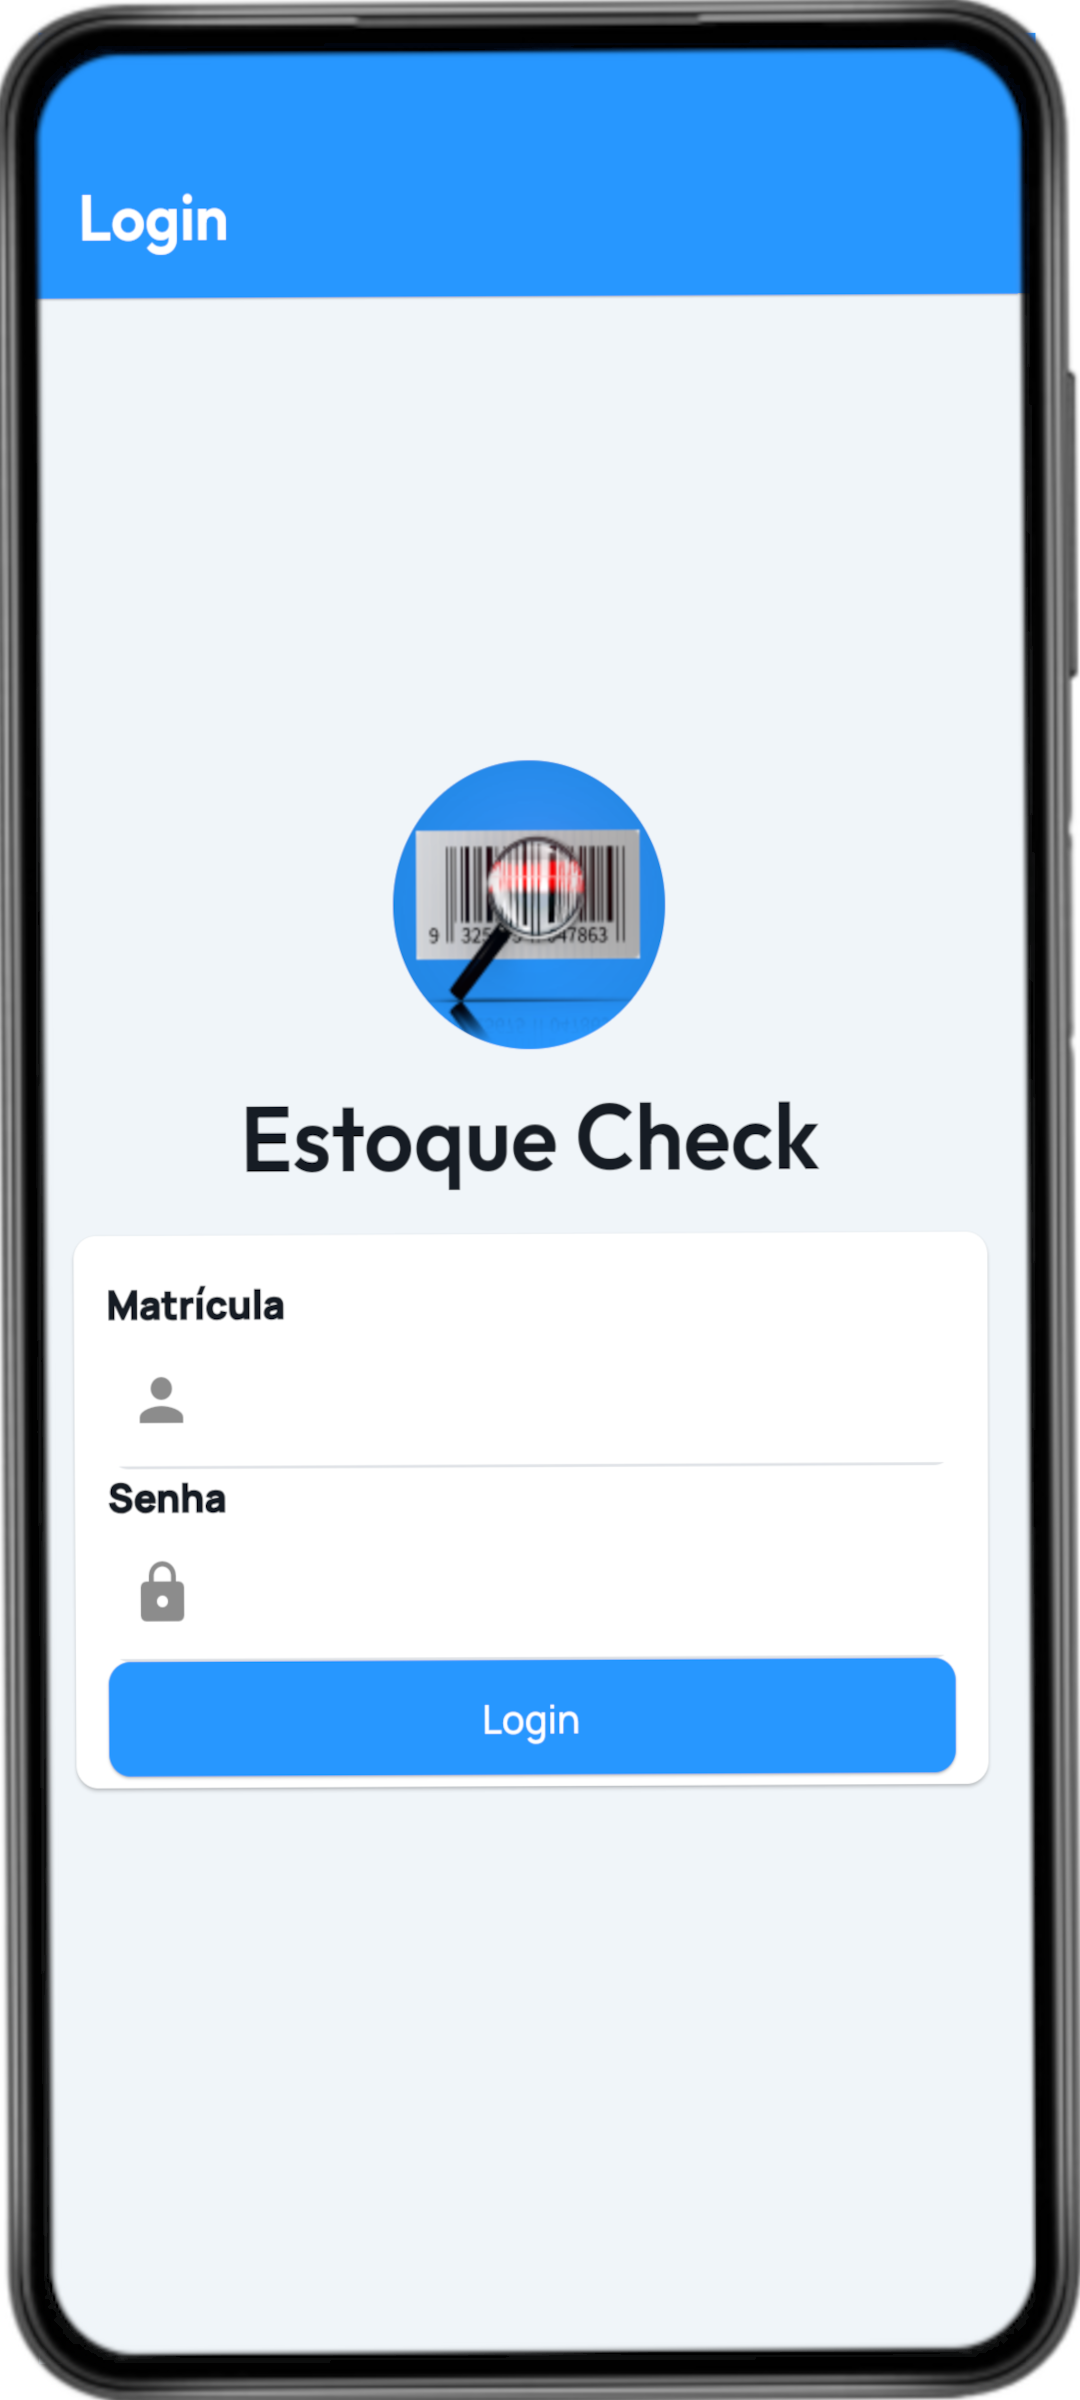
\includegraphics[width=0.15\textwidth]{imgs/login.png}
    }
    \quad
    \subfigure[Tela principal.]{
        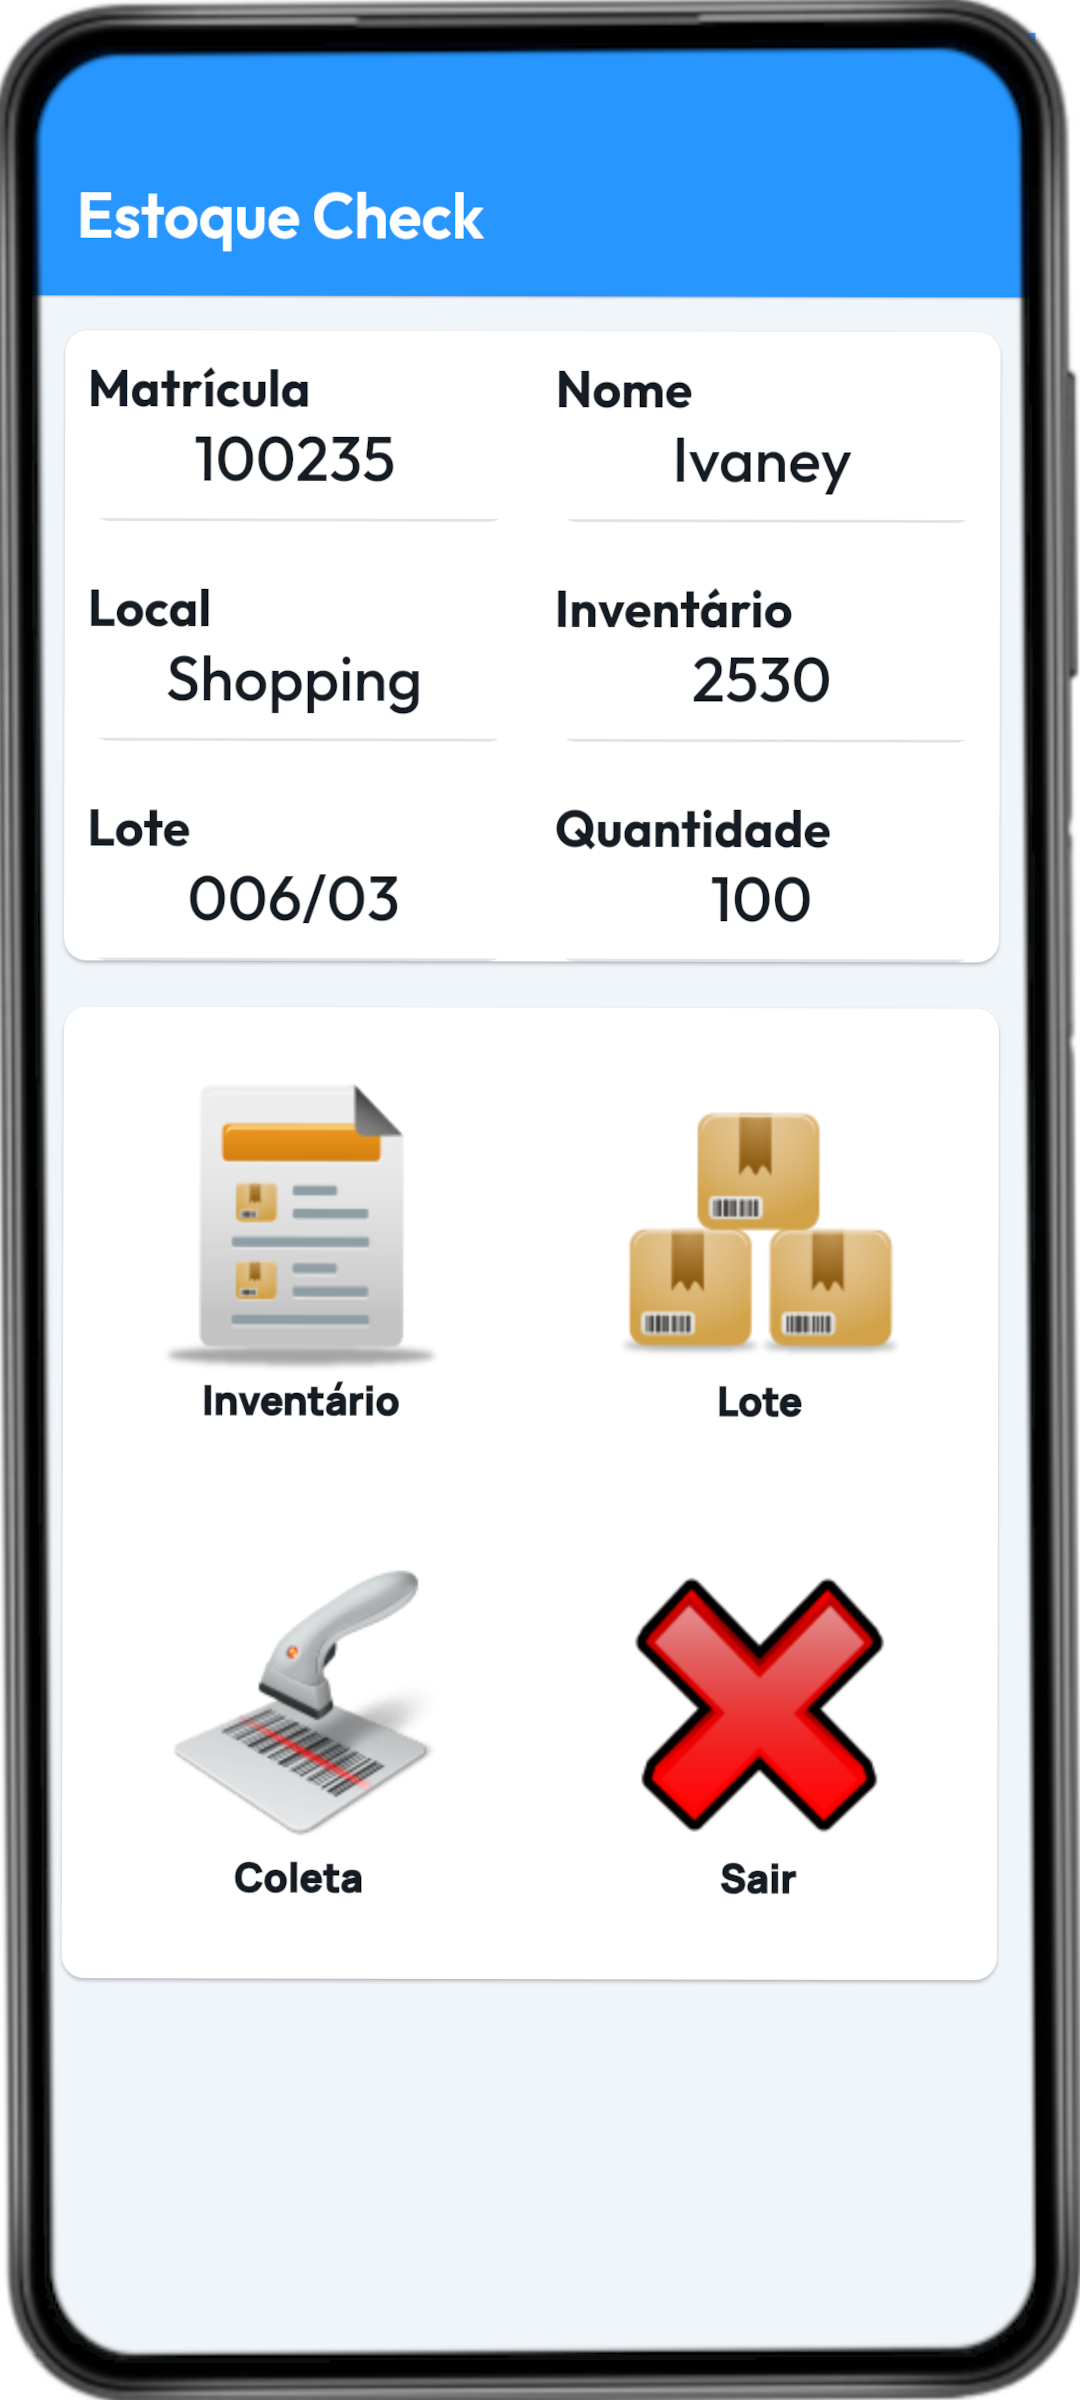
\includegraphics[width=0.15\textwidth]{imgs/homepage.png}
    }
    \quad
    \subfigure[Seleção de inventário.]{
        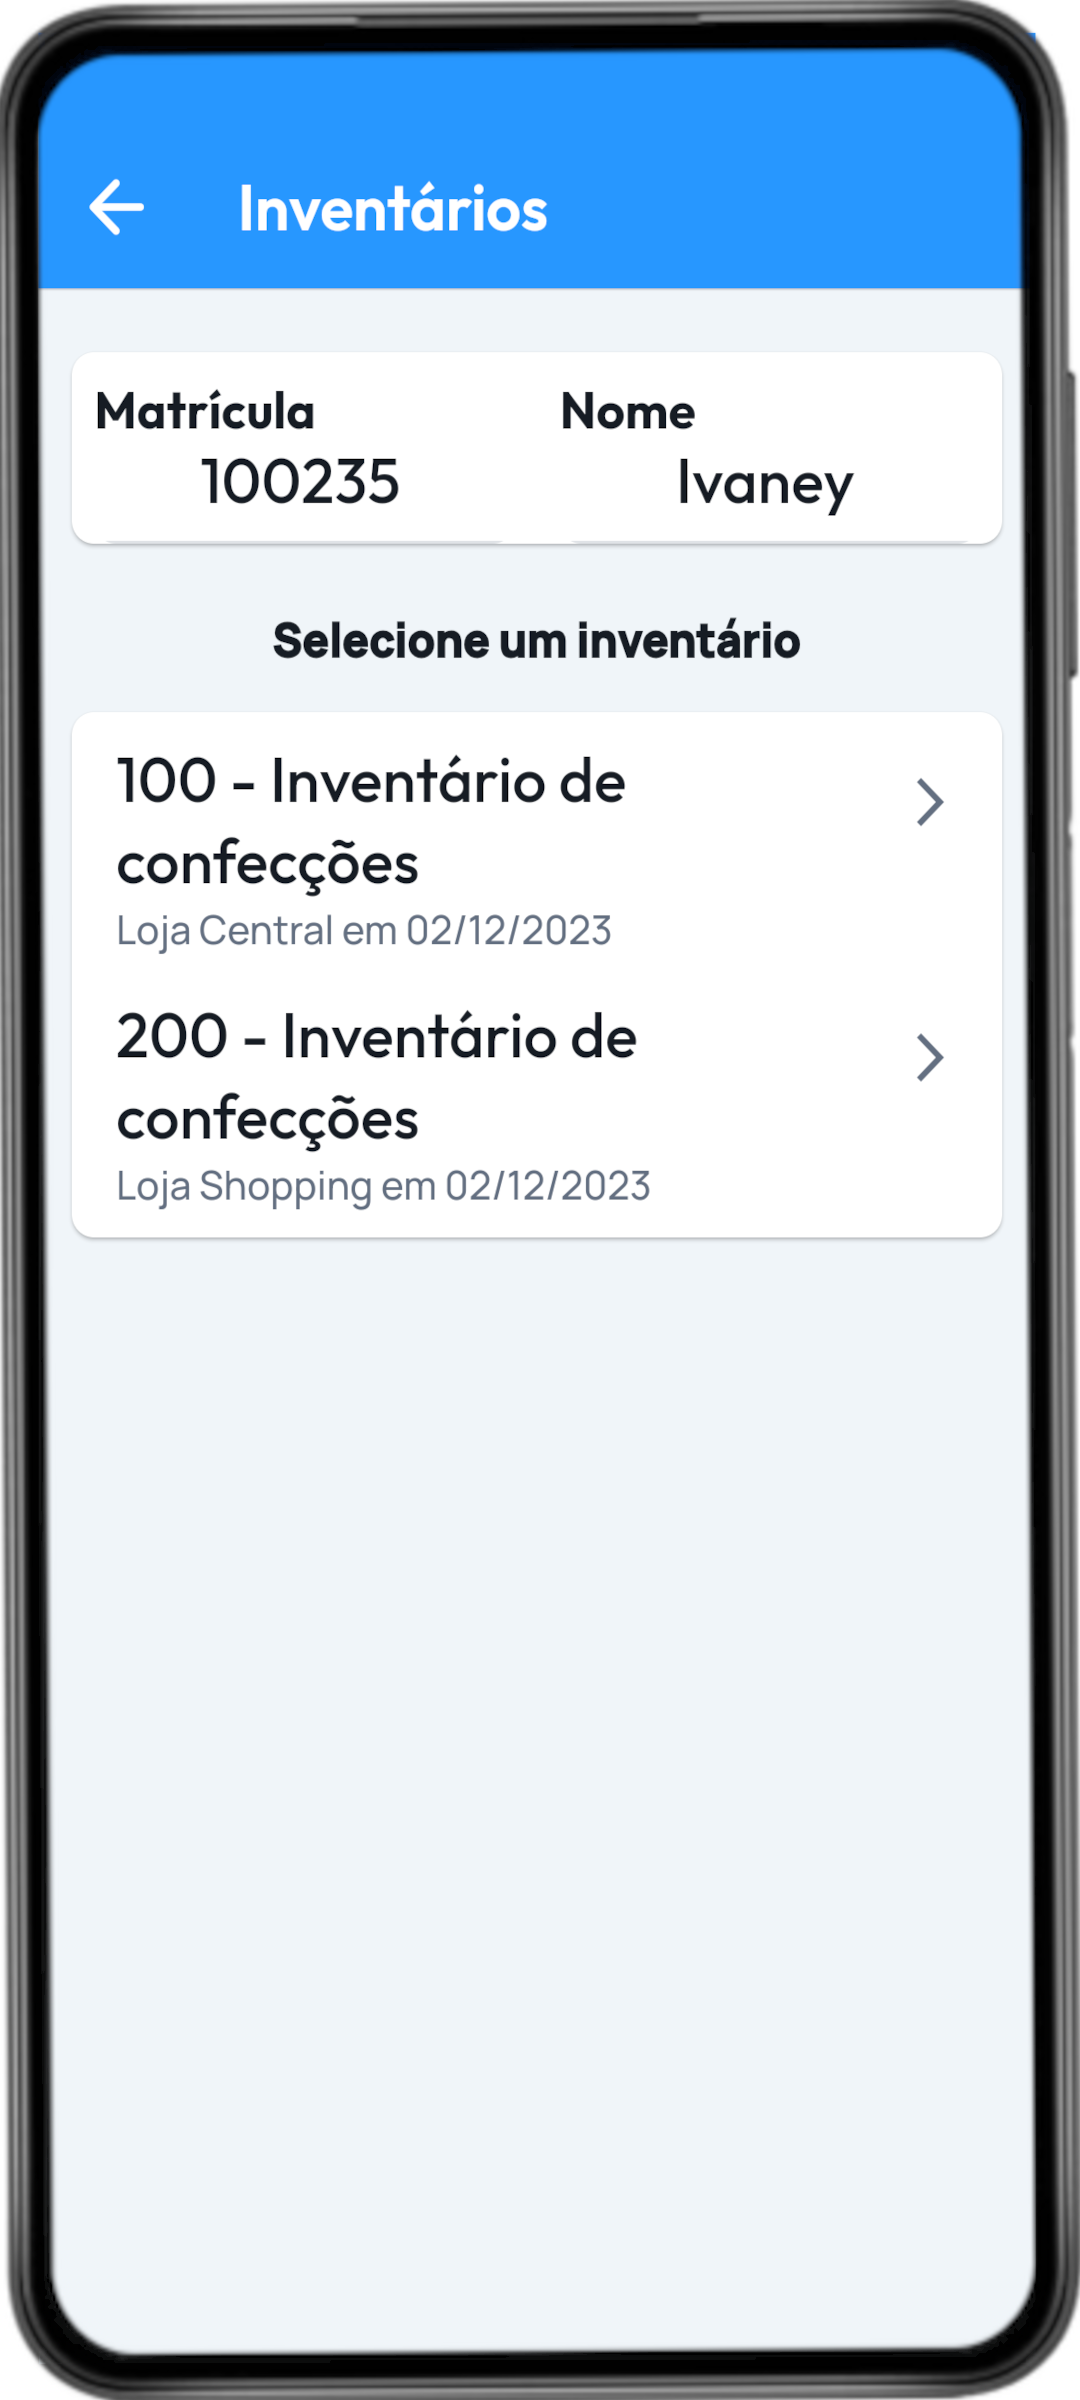
\includegraphics[width=0.15\textwidth]{imgs/inventario.png}
    }
    \quad
    \subfigure[Seleção de lote.]{
        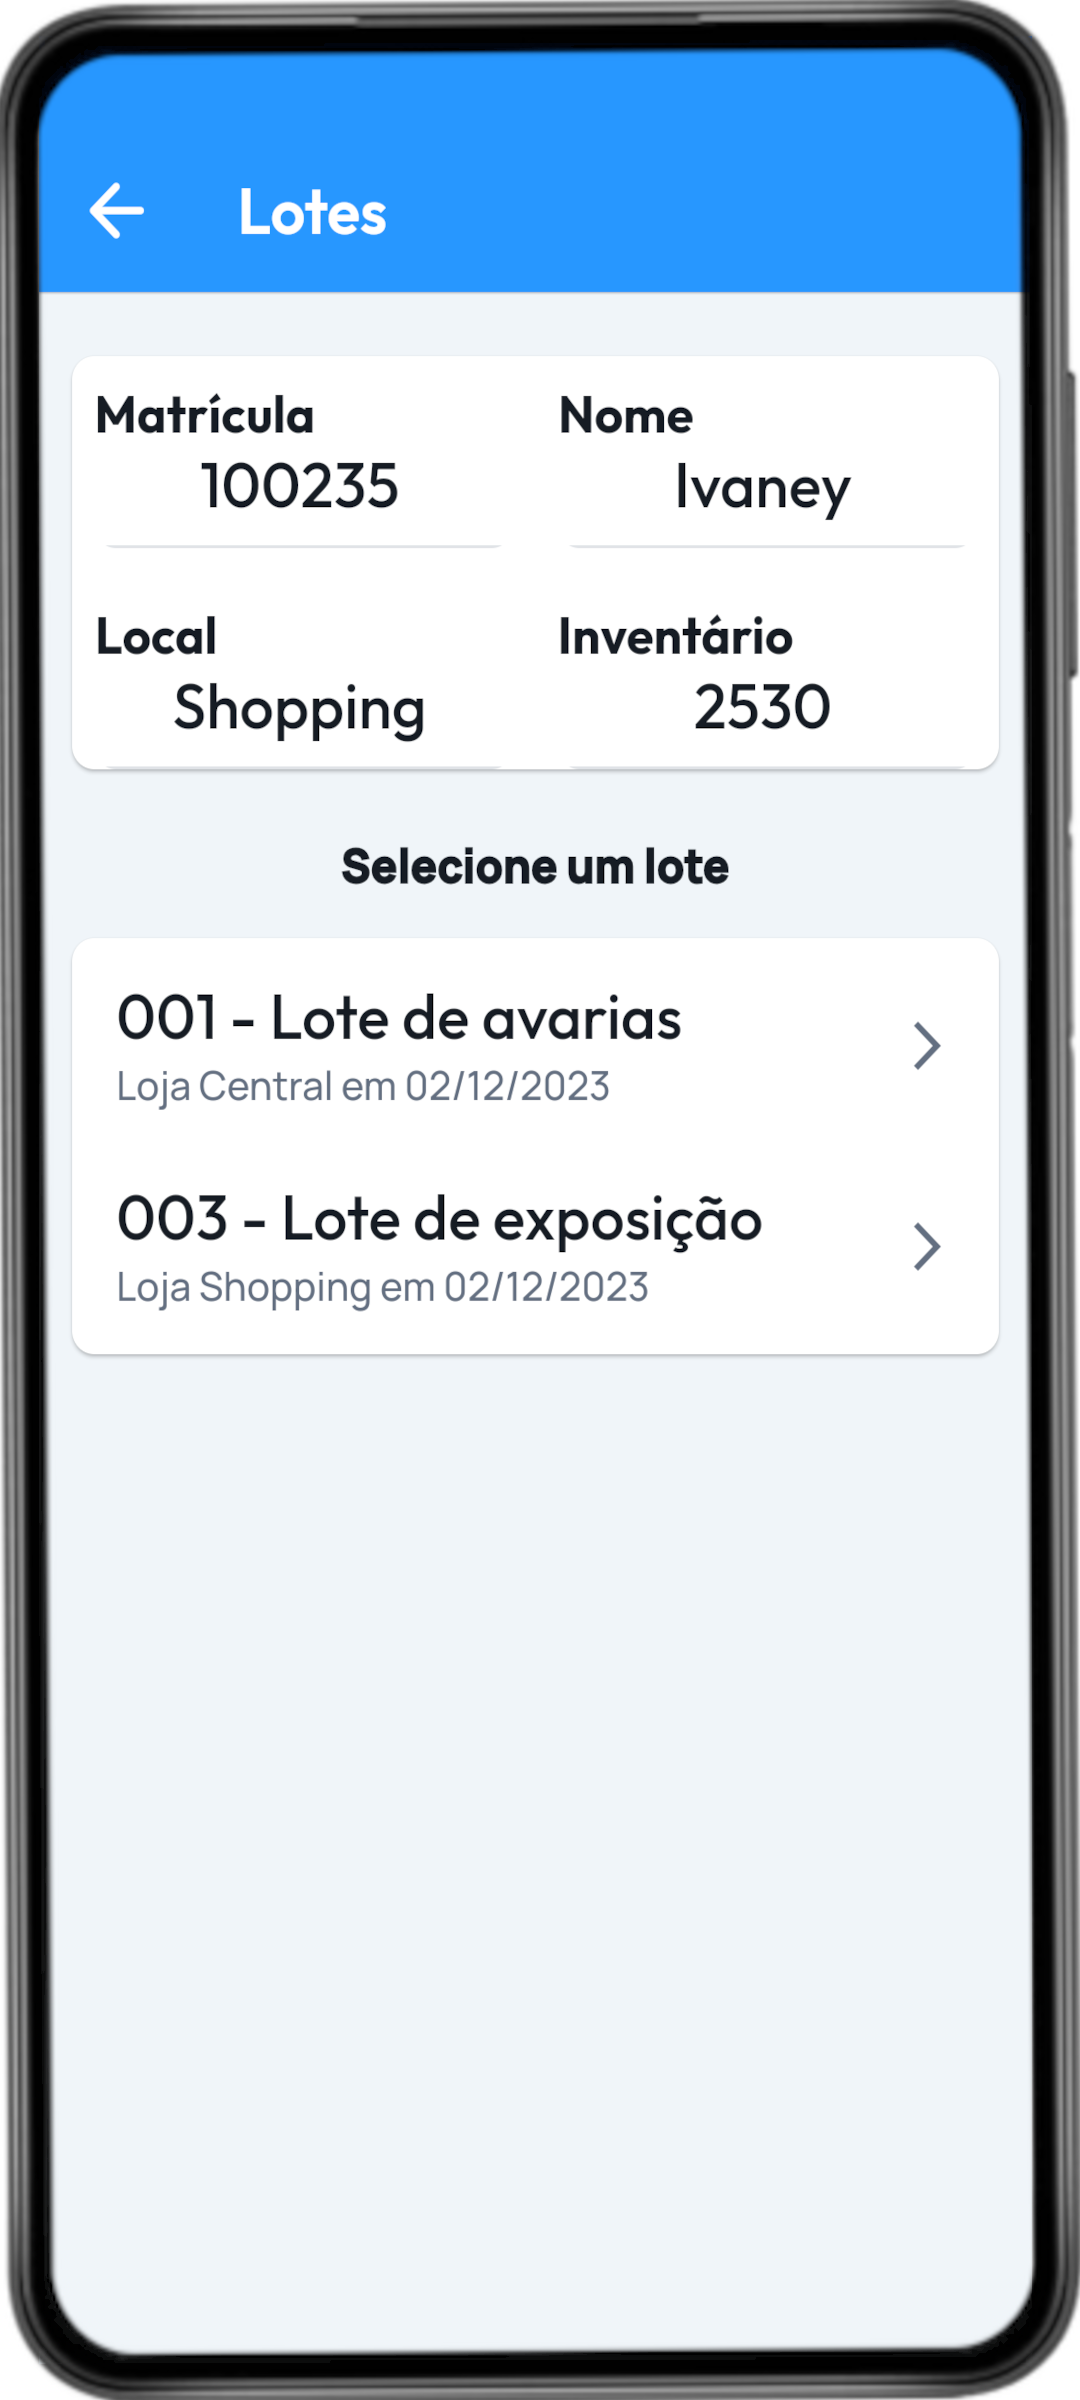
\includegraphics[width=0.15\textwidth]{imgs/lote.png}
    }
    \quad
    \subfigure[Coleta para contagem.]{
        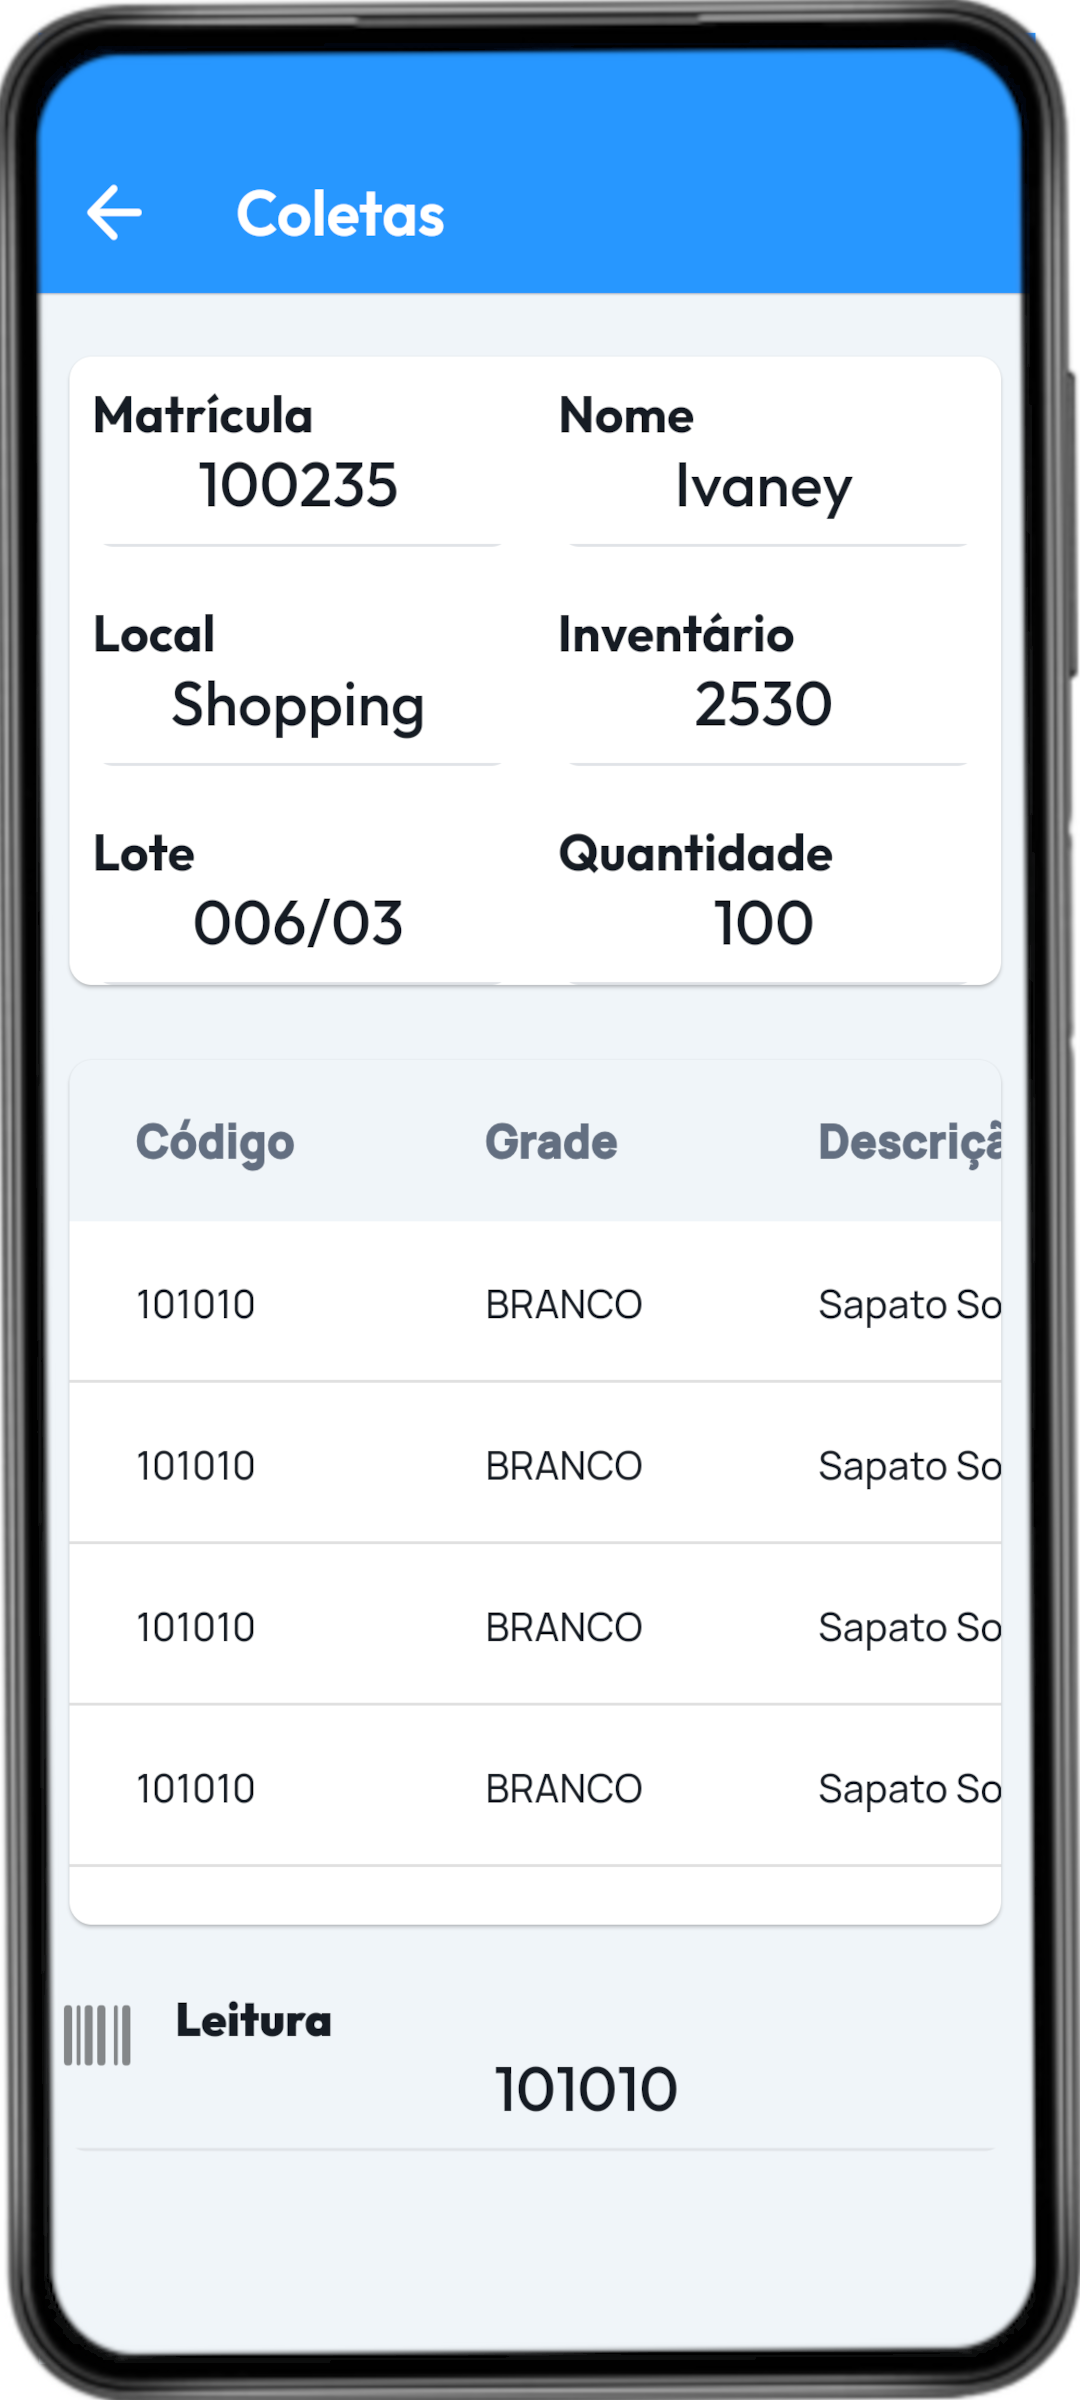
\includegraphics[width=0.15\textwidth]{imgs/coleta.png}
    }
    \caption{Layout de telas para o aplicativo}
    \label{fig:telas}
\end{figure}

A figura \ref{fig:telas} apresenta o layout das telas do aplicativo conforme descrito a seguir:

\begin{itemize}
    \item \textbf{Tela de Login}: Esta tela destina-se à autenticação do usuário no aplicativo. O usuário deve inserir seu nome de usuário e senha válidos, que correspondem às credenciais de acesso do sistema de gestão da empresa.

    \item \textbf{Tela Principal}: A tela principal apresenta ao usuário as opções para iniciar uma nova contagem de inventário ou retomar uma contagem já em andamento.

    \item \textbf{Seleção de Inventário}: Nesta tela, o usuário visualiza a lista de inventários disponíveis para contagem e seleciona aquele que deseja realizar o procedimento.

    \item \textbf{Seleção de Lote}: A tela de seleção de lote apresenta ao usuário a lista de lotes disponíveis dentro do inventário escolhido. O usuário deve selecionar o lote que deseja contar. Um lote é definido como um conjunto de produtos agrupados em um espaço físico específico, como um palete, uma gôndola ou uma estante. Cada lote é identificado por um código e um código de barras. O auditor pode selecionar o lote desejado lendo o código de barras com o coletor.

    \item \textbf{Coleta para Contagem}: Nesta tela, o usuário visualiza os produtos presentes no lote selecionado e registra a quantidade contada de cada item. Ao finalizar a contagem, os dados coletados são enviados ao sistema de gestão da empresa. Nesse momento, o status do lote é atualizado para “fechado”, podendo ser reaberto apenas pelo administrador do sistema.
\end{itemize}

Durante a contagem, o administrador monitora o progresso das contagens por meio de um dashboard e pode configurar alertas para serem enviados aos auditores, informando sobre a proximidade do término do inventário ou eventuais atrasos na contagem.

Após a conclusão da contagem, o administrador fecha o inventário. Os dados são validados por meio de uma análise estatística e, em seguida, processados para realizar ajustes gerenciais e fiscais do estoque.

\subsection{Aplicativos semelhantes}

A tabela \ref{tab:comparativos} uma comparação entre os aplicativos IS Collector, KCollector e Stock e Inventário Simples, que são aplicativos de contagem de inventário disponíveis na loja de aplicativos do Google. A análise abrange suas principais funcionalidades.

\begin{table}[!htb]
    \centering
    \caption{Funcionalidades dos aplicativos semelhantes.}
    \label{tab:comparativos}
    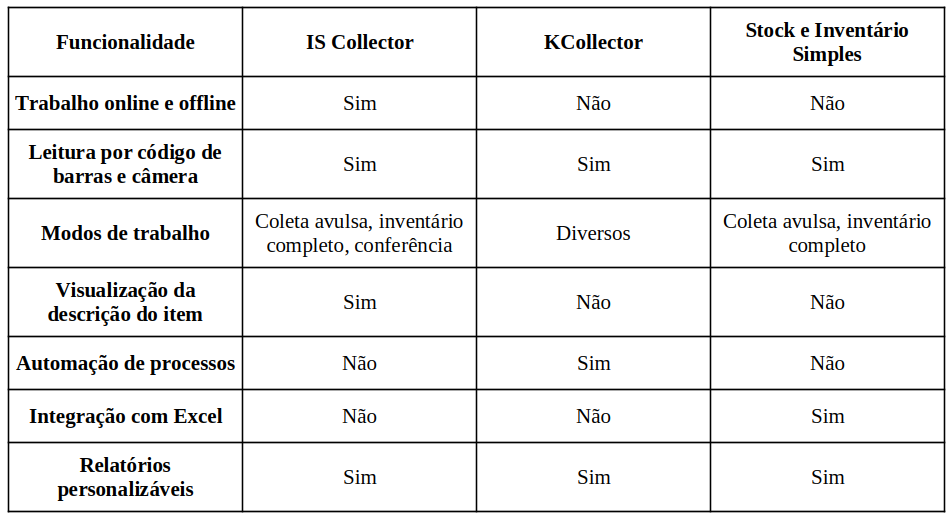
\includegraphics[width=1.0\textwidth]{tables/comparativo.png}
    %Fonte: \cite{googleplay}.
\end{table}

O IS Collector se destaca pela flexibilidade e abrangência de funções, ideal para empresas que exigem um alto nível de controle e automação no processo de inventário. O KCollector é a opção ideal para quem busca uma solução acessível e prática, que transforma o celular em um coletor eficiente. Já o Stock e Inventário Simples se destaca pela facilidade de uso e pelo gerenciamento completo do estoque, sendo uma ótima opção para iniciantes e pequenos negócios.

% Colocar aqui um parágrafo comparando o aplicativo do trabalho com os aplicativos pesquisados
O aplicativo do presente trabalho se destaca pela integração com o sistema de gestão da empresa, garantindo a consistência e a atualização em tempo real dos dados de estoque. Além disso, a interface intuitiva e as funcionalidades customizáveis proporcionam uma experiência de usuário eficiente e adaptável às necessidades específicas de cada empresa. A integração com tecnologias avançadas, como leitura de códigos de barras e alerta automatizados, eleva a eficácia do aplicativo, tornando-o uma solução completa e moderna para o controle de inventário.


\section{Considerações finais}

%O inventário não deve ser encarado apenas como uma correção pontual, mas como um processo contínuo e integrado à gestão operacional. A implementação de tecnologias avançadas, como sistemas automatizados de rastreamento e leitura por código de barras, pode elevar ainda mais a eficácia desse processo, reduzindo o tempo necessário para identificar e corrigir discrepâncias.
%
%Em resumo, o problema dos erros de estoque no varejo brasileiro é uma realidade desafiadora, mas o investimento em um processo de inventário robusto emerge como uma solução estratégica e proativa. Ao adotar essa abordagem, os varejistas não apenas minimizam as falhas operacionais, mas também fortalecem a base para uma gestão de estoque eficiente e uma experiência de compra mais satisfatória para os clientes.
%
%Os resultados apresentados reforçam a importância de um sistema de inventário bem-estruturado para a eficiência operacional e a satisfação do cliente. A implementação de tecnologias como o Flutter para o frontend e o Spring Boot para o backend demonstra a viabilidade de soluções tecnológicas modernas na gestão de inventários, oferecendo uma base sólida para a automação e otimização dos processos.

Os erros de saldo de estoque no varejo brasileiro são um desafio significativo que afeta a eficiência operacional e a satisfação do cliente. Este trabalho propõe um processo de inventário robusto e contínuo, integrado à gestão operacional, como solução estratégica.

A adoção de tecnologias avançadas, como sistemas automatizados de rastreamento e leitura por código de barras, pode aumentar a eficácia do processo, reduzindo o tempo para corrigir discrepâncias. Ferramentas como Flutter e Spring Boot demonstram a viabilidade de criar sistemas eficientes para a gestão de inventários.

Entretanto, a tecnologia sozinha não resolve todos os problemas. É crucial ter processos bem definidos, treinamento adequado e uma cultura organizacional que valorize a precisão. Assim, ao adotar essas práticas, os varejistas não apenas minimizam os erros de saldo de estoque, mas também melhoram a gestão de estoque e a experiência de compra para os clientes.

% Referencia \cite{silva2022}.

\bibliographystyle{sbc}
\bibliography{bibliografia}


\end{document}
